\documentclass[../main.tex]{subfiles}
\graphicspath{{\subfix{../images/}}}

\begin{document}
	\chapter{Struttura dell'azienda e del suo sistema informativo}
	\section{Concetto di esigenza informativa}
	La funzione principale di un sistema informativo è di interagire, aiutandi, ogni figura professionale che fa funzionare l'azienda.\\
	E' importante fare due distinzioni di ruoli:
	\begin{enumerate}
		\item \textbf{Esecutivo}
		\item \textbf{Direttivo}
	\end{enumerate}
	Queste due tipologie di ruoli hanno bisogno di informazioni diverse e quindi le informazioni verranno date in modo meno o più astratto.
	\begin{itemize}
		\item I ruoli esecutivi avranno bisogno di informazioni molto specifiche della situazione attuale.
		\item I ruoli dirigenziali invece avranno a disposizione dei dati che forniscono una visione molto più ampia ma sono più sintetici.
	\end{itemize}
	All'interno del sistema informativo aziendale devono quindi coesistere i dettagli richiesti dai ruoli operativi e la sintesi richiesta dai dirigenti.

	\subsection{Schema di Anthony}
	Come abbiamo visto cambiando di mansione cambiano anche i dati che risultano utili.\\
	Ma come si può identificare a che dipendenti vanno fornite certe informazioni?\\
	Il modello di Anthony propone di distinguere le mansioni in tre livelli, ogni livello interagisce con gli adiacenti mediante cicli di verifica delle informazioni.
	\begin{enumerate}
		\item \textbf{Direzionale strategico:} identifica gli obiettivi principali a medio-lungo termine.
		\item \textbf{Direzionale tattico:} che compie analisi economiche ponendo obbiettivi a medio termine, inoltre fornisce gli indirizzi operativi ai settori esecutivi.
		\item \textbf{Operativo:} attua i piani definiti.
	\end{enumerate}
	\begin{center}
		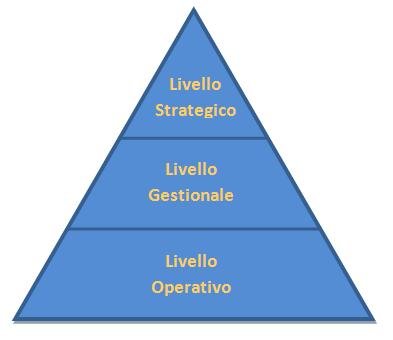
\includegraphics[scale=0.5]{anthony_mark_01.jpg}
	\end{center}

	\subsection{Profili informativi}
	\subsubsection{Livello direzionale strategico}
	A questo livello competono informazioni sintetiche, molto diversificate e poco strutturate.\\
	Al decisore deve essere affiancato un sistema informativo in grado di mostrare:
	\begin{itemize}
		\item indicatori prestazionali dell'azienda.
		\item evoluzioni delle strategie adottate in precedenza.
		\item scenari fittizzi per simulazioni.
		\item ogni tipo di indicatore sulla salute dell'azienda.
	\end{itemize}

	\subsubsection{Livello direzionale tattico}
	Il livello tattico si occupa di tutte quelle attività di definizione di obbiettivi a breve termine che rispettino le strategie aziendali e il periodico controllo dei risultati.\\
	Le informazioni necessarie sono ottenute sintetizzando i dati estratti dai sistemi di supporto al livello operativo.

	\subsubsection{Livello operativo}
	In questo livello ci si occupa dell'attuazione dei piani e delle attività correlate.

	\subsubsection{Tabella riassuntiva}
	\begin{center}
		\begin{tabular}{|l|c|c|c|c|}
			\hline
			& \textbf{Frequenza} & \textbf{Dati} & \textbf{Provenienza} & \textbf{Volumi}\\
			\hline
			\textbf{\begin{tabular}{@{}c@{}} Livello \\ direzionale \\ strategico \end{tabular}} & casuale & \begin{tabular}{@{}c@{}} sintetici e\\ non strutturati \end{tabular} & interna ed esterna & bassi\\
			\hline
			\textbf{\begin{tabular}{@{}c@{}} Livello \\ direzionale \\ tattico \end{tabular}} & prefissata & sintetici o analitici & interna & medi\\
			\hline
			\textbf{\begin{tabular}{@{}c@{}} Livello \\ operativo \end{tabular}} & costante & analitici & interna & elevati\\
			\hline
		\end{tabular}
	\end{center}

	\section{Scomposizione del sistema informativo}
	Le diverse esigenze tra i  vari livelli ha portato, nel tempo, ad una separazione tra i sistemi informativi.\\
	Si sono venuti a creare due tipologie di sistemi:
	\begin{enumerate}
		\item \textbf{Sistemi informazionali:} che aiutano nella risoluzione di problemi che non sempre hanno una struttura precisa, vengono alimentati con i dati raccolti dai sistemi operazionali.\\
			Negli anni si sono evoluti per collezioanre in modo sempre più rapido ed efficente l'andamento azziendale e quello della concorrenza.
		\item \textbf{Sistemi operazionali:} hanno una strattura fissa e molto rigida, infatti svolgono il mestiere per il quale vengono pensati, non sono più di aiuto quando si voglia percorrere un percorso di risoluzione diverso.
	\end{enumerate}
	\begin{center}
		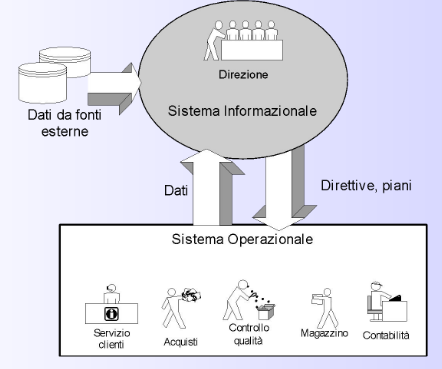
\includegraphics[scale=0.6]{relazione_sistemi_operazionale_informazionale.png}
	\end{center}
	Questa separazione rompe però la struttura di Anthony che può essere riopensata come:
	\begin{center}
		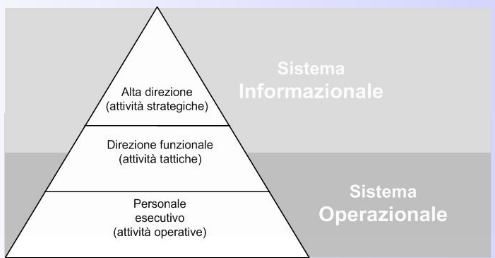
\includegraphics[scale=0.5]{anthony_mark_02.png}
	\end{center}

	\subsection{Sistemi operazionali}
	Le principali funzioni di un sistema operazionale sono:
	\begin{itemize}
		\item L'automatizzazione di attività procedurali, in cui il sistema simula un impiegato, un esempio può essere la compilazione automatica delle fatture.
		\item L'aiuto per le attività aziendali, il sitema operazionale deve rendere di facile accesso e modifica i dati.
		\item La raccolta i dati necessari ai livelli decisionali per il controllo delle attività.
		\item La guida del'operatore attraverso un flusso di operazioni da compiere.
	\end{itemize}
	Dato il suo scopo operativo, il sistema operazionale tende a creare strutture per i flussi standard per cercare di minimizzare la possibilità di errore e rendere le operazioni facili e veloci.\\
	Spesso i sistemi informativi devono interagire con delle basi di dati, per cui per un sistema operazionale è necessario che:
	\begin{itemize}
		\item Le procedure con le quali si guida l'operatore.
		\item Che la base di dati sia performante per poter vedere consultare/modificare i dati velocemente.
	\end{itemize}
	Il sistema operazionale deve poter performare delle operazioni sui dati, le operazioni possono essere:
	\begin{itemize}
		\item Acesso e modifica in tempo reale.
		\item Trattamento dei dati.
		\item Descrizione di eventi, come transazioni economiche.
		\item Valutazione e trattamento dei dati attuali.
		\item Aggregazione di indicatori di stato.
	\end{itemize}
	\subsection{Sistemi informazionali}
	I processi decisionali non sono standard e perciò è impossibile creare modelli della realtà che le persone possano seguire.\\
	Infatti le esigenze che deve soddisfare un sistema informazionale sono:
	\begin{itemize}
		\item Risultati rispetto agli obbiettivi prefissati.
		\item Struementi per il confronto tra indicatori di più aziende.
		\item Strumenti che facilitino il processo decisionale, come analisi interattiva o ricerca di correlazione tra i dati.
	\end{itemize}
	La natura delle informazioni direzionali è totalmente divresa, infatti prevede quanto segue.
	\begin{itemize}
		\item L'aggregazione di dati con decisioni basate su informazioni statistiche.
		\item La profondità temporale, per valutare l'andamento dei dati in un periodo di tempo.
		\item La ricerca per argomento.
		\item L'analisi multidimensionale, infatti per i processi decisionali è fondamentale poter incrociare le informazioni.
	\end{itemize}
	Il punto focale dei sistemi informazionali è la base di datai che assumen il nome di "data warehouse" che deve essere:
	\begin{itemize}
		\item Altamente centralizzato.
		\item Strutturato per poter ospitare tutti i dati utili all'analisi.
		\item Aggiornato costantemente con dati coerenti e completi.
		\item Permanente.
		\item Facile da interrogare.
	\end{itemize}
	Questi sistemi hanno due parti fondamentali al loro interno, ovvero:
	\begin{enumerate}
		\item Le procedure di alimentazione, che garantiscono la qualità e la completezza dei dati provenienti dai processi decisionali.
		\item I sistemi di analisi e presentazione dell'informazione.
	\end{enumerate}

	\subsection{Comparazione tra sistemi operazionali e informazionali}
	Come è facile intuire le levate differenze tra i sistemi informativi ha portato alla nascita di sistemi differenti, in base al contesto.\\
	I sistemi operazionali si sono dimostrati anche insufficienti da alcuni punti di vista prestazionali, per cui si è deciso di optare per la suddivisione in due categorie:
	\begin{enumerate}
		\item \textbf{OLTP(OnLine Transaction Processing):} indicano un gruppo di sistemi che trattano le transazioni, ottimizzati per garantire la massima responsività nella gestione dei processi operativi aziendali.\\
			Puntano soprattutto per garantire ad una vasta larga di utenti simultanei l'accesso veloce alla base di dat.
		\item \textbf{OLAP(OnLine Analytical Processing):} sono il sottoinsieme di sistemi pensati per l'analisi dei dati, sono ottimizzati per garantire le massime prestazioni nell'elaborazione dei dati sintetici e nelle interrogazioni.
	\end{enumerate}

	\subsubsection{Tabella riassuntiva}

	\begin{center}
		\begin{tabular}{|c|c|c|}
			\hline
			& \textbf{OLTP} & \textbf{OLAP}\\
			\hline
			\textit{Finalità} & Supporto all'operatività & Supporto al processo decisionale\\
			\hline
			\textit{Utenti} & Molti, operativi & Pochi, direzionali\\
			\hline
			\textit{Dati} & Analitici & Sintetici, spesso numerici\\
			\hline
			\textit{Modalità di utilizzo} & Guidata & Interrogazioni ad hoc\\
			\hline
			\textit{Quantità di dati} & Bassa(centinaia di record) & Alta(Milioni di record)\\
			\hline
			\textit{Orientamento} & Per processi/applicazioni & Per area/tema\\
			\hline
			\textit{Frequanza di aggiornamento} & Continua & Sporadica, esplicita\\
			\hline
			\textit{Copertura temporale} & Dati correnti & Storica\\
			\hline
			\textit{Ottimizzazione} & Per accessi di lettura e srittura & Per accessi in lettura e aggregazione\\
			\hline
		\end{tabular}
	\end{center}
\end{document}